\subsection*{Обобщение на случай отражения}

В прошлый раз у нас было матрица $T$ \eqref{t-matrix} и матрица $P$ \eqref{p-matrix}.

\begin{figure}[htb]
	\centering
	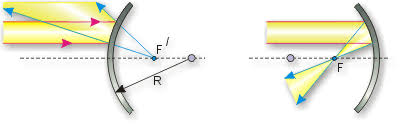
\includegraphics{img/otrazenie.png}
\end{figure}

Возьмём теперь зеркало, посмотрим на отражение для выгнутого зеркала (слева) и напишем матрицу отражения.
\begin{equation*}
	n_1 = n, n_2 = -n
	\hspace{0.5 cm}
	\leadsto
	\hspace{0.5 cm}
	R = \begin{pmatrix}
		1 & 0 \\ -\dfrac{- n -n}{R} & 1
	\end{pmatrix}
	=
	\begin{pmatrix}
		1 & 0 \\ \dfrac{2n}{R} & 1
	\end{pmatrix}
\end{equation*}
для вогнутого же (справа) заодно выпишем сразу все матрицы, которые у нас есть:
\begin{equation*}
	R = \begin{pmatrix}
		1 & 0 \\ -\dfrac{2n}{R} & 1
	\end{pmatrix}
	\hspace{1 cm}
	P= \begin{pmatrix}
		1 & 0 \\ -\dfrac{n_2 - n_1}{R} & 1
	\end{pmatrix}
	\hspace{1 cm}
	T = \begin{pmatrix}
		1 & l/n \\
		0 & 1
	\end{pmatrix}
\end{equation*}

\subsubsection*{Пример 1}
Допустим шёл луч и упал на плоскопараллельную пластину и пошёл внутри неё змейкой.
\begin{equation*}
	\begin{pmatrix}
		1 & h/n \\ 0 & 1
	\end{pmatrix}
	=
	\begin{pmatrix}
		1 & h N/n \\ 0 & 1
	\end{pmatrix}
\end{equation*}

\subsubsection*{Задача 13}
Описываем жизнь нашего  луча умножением матриц:
\begin{equation*}
	\begin{pmatrix}
		1 & 0 \\ -\dfrac{n-1}{R} & 1
	\end{pmatrix}
	\begin{pmatrix}
		1 & \dfrac{2R}{n} \\ 0 & 1
	\end{pmatrix}
	\begin{pmatrix}
		1 & 0 \\ -\dfrac{2n}{R} & 1
	\end{pmatrix}
	\begin{pmatrix}
		1 & \dfrac{2 R}{n} \\ 0 & 1
	\end{pmatrix}
	\begin{pmatrix}
		1 & 0 \\ -\dfrac{n-1}{R} & 1
	\end{pmatrix}
	= 
	\begin{pmatrix}
		\dfrac{n-4}{n} & -\dfrac{4 R}{n} \\ \dfrac{2(n-2)}{n R} & \dfrac{n-4}{n}
	\end{pmatrix}
\end{equation*}

\subsection*{Периодические оптические системы}
Пусть у нас оптическая ячейка уже после перемножения всех матриц характеризуется в итоге матрицей 2х2, с элементами $A, B, C, D$.
У периодической системы такая ячейка встречается $m$ раз:
\begin{equation*}
	\begin{pmatrix}
		y_m \\ v_m
	\end{pmatrix}
	=
	\begin{pmatrix}
		A & B \\ C & D
	\end{pmatrix}^m
	\begin{pmatrix}
		y_0 \\ v_0
	\end{pmatrix}
	\hspace{0.5 cm}
	\leadsto
	\hspace{0.5 cm}
	\begin{pmatrix}
		y_{m+1} \\ v_{m+1}
	\end{pmatrix}
	=
	\begin{pmatrix}
		A & B \\ C & D
	\end{pmatrix}^m
	\begin{pmatrix}
		y_m \\ v_m
	\end{pmatrix}
\end{equation*}
Получаем уравнения:
\begin{equation*}
\left\{
	\begin{aligned}
		&y_{m+1} = A y_m + B v_m \\
		&v_{m+1} = C y_m + D v_m
	\end{aligned}
\right.
	\hspace{0.5 cm}
	\Rightarrow
	\hspace{0.5 cm}
\left\{
	\begin{aligned}
		&v_m = \frac{y_{m+1} - A y_m}{B} 
		\hspace{0.2 cm}
		\Rightarrow
		\hspace{0.2 cm}
		v_{m+1} = \frac{y_{m+2} - A y_{m+1} }{B} \\
		&y_{m+2} - A y_{m+1} = B C y_m +D(y_{m+1} - A y_m)
	\end{aligned}
\right.
\end{equation*}
Получили уравнение на $y$:
\begin{equation*}
	y_{m+2} - (A + D) y_{m+1} + (A D - B C) y_m = 0
	\hspace{0.3 cm}
	\Rightarrow
	\hspace{0.3 cm}
	y_m = y_0 h^m
	\hspace{0.3 cm}
	\Rightarrow
	\hspace{0.3 cm}
	h^2 - (A + D)h + 1 = 0	
\end{equation*}
Заменяя $A+D = 2b$, получаем три случая на детерминант: $h_{1,2} = b \pm \sqrt{b^2 - 1}$.
\begin{enumerate}
	\item $|b|<1$: Тогда $h_{1,2} = e^{i \varphi}$ $\Rightarrow$ $y_m = \alpha_1 e^{i m \varphi} + \alpha_2 e^{- i m \varphi} = y_{\text{max}} \sin (m \varphi + \varphi_0)$.
\end{enumerate}
Заметим, что $y_m$ периодичен, только если $\varphi/2\pi$ -- рациональное число.

\subsubsection*{Пример 2}
Дана система линз: $\uparrow-d-\uparrow-d-\uparrow$. Матрицы прохождения луча:
\begin{equation*}
	\begin{pmatrix}
		1 & 0 \\ -1/F & 1
	\end{pmatrix}
	\begin{pmatrix}
		1 & d \\ 0 & 1
	\end{pmatrix}
	=
	\begin{pmatrix}
		1 & d \\ -1/F & 1 - d/F
	\end{pmatrix}
\end{equation*}
Получаем, что устойчиво когда:
\begin{equation*}
	b = \frac{2- d/F}{2}
	\hspace{0.3 cm}
	\leadsto
	\hspace{0.3 cm}
	|b|<1
	\hspace{0.3 cm}
	\leadsto
	\hspace{0.3 cm}
	0 < \frac{b}{F} < 4.
\end{equation*}
Посмотрим случаи:
\begin{enumerate}
	\item $d = F$: тогда $b = 1/2$, и тогда $b = \cos \varphi \Rightarrow \varphi = \frac{\pi}{3}$;
	\item $d = 2 F$: тогда $b=0$;
	\item $d = 0$: тогда $d = 4F$.
\end{enumerate}

\subsection*{Оптический резонатор}
Пусть у нас есть два зеркала: $\big(-L-\big)$. Матрица:
\begin{equation*}
	\begin{pmatrix}
		1 & 0 \\ 2/R_2 & 1
	\end{pmatrix}
	\begin{pmatrix}
		1 & L \\ 0 & 1
	\end{pmatrix}
	\begin{pmatrix}
		1 & 0 \\ 2/R_1 & 1
	\end{pmatrix}
	\begin{pmatrix}
		1 & L \\ 0 & 1
	\end{pmatrix}
	\hspace{0.5 cm}
	\Rightarrow
	\hspace{0.5 cm}
	b = (A + D)/2 = 2 \underbrace{\left(1 + \frac{L}{R_1}\right)}_{g_1} \underbrace{\left(1 + \frac{L}{R_2}\right)}_{g_2} - 1.
\end{equation*}
Можно рассмотреть различные типы резонаторов:
\begin{enumerate}
	\item Плоский;
	\item Симметричный конфокальный;
	\item Симметричный концентрический.
\end{enumerate}